\graphicspath{ {./images/7_Glycosylation_traits} }
\newpage

\section{Glycosylation traits (optional)}
Glycosylation traits can be calculated automatically for human IgG, IgA and IgM (including Joining Chain), and for mouse IgG.
These calculations rely on a reference list containing glycan compositions with known structures, listed in appendix \ref{glycan_compositions}.
If your curated data contains glycan compositions that are not listed there, there is an option to calculate glycosylation traits manually.

\subsection{Calculate traits automatically}
To calculate glycosylation traits automatically, start by selecting the type of glycans that are present in your data.
Then choose the traits that you wish to calculate.
For each desired trait, enter the glycosylation sites in your data for which they should be calculated.
Then click the \menu{Calculate traits} button.
\begin{center}
	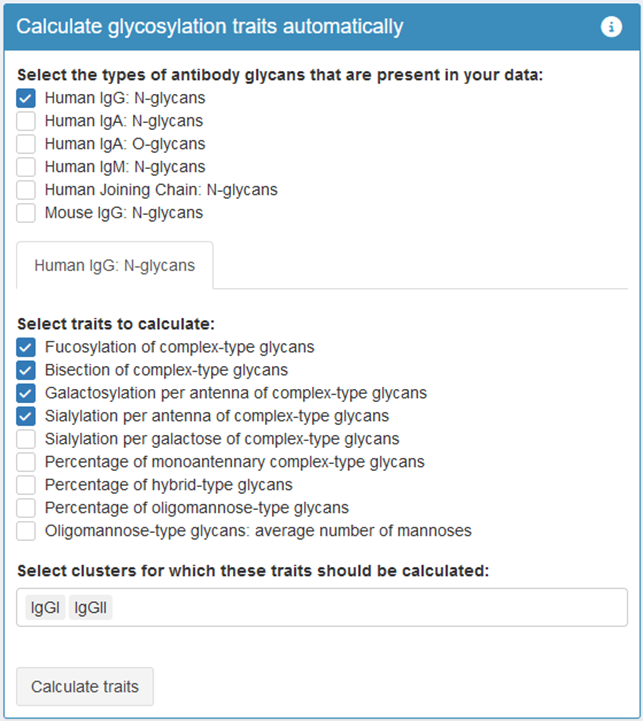
\includegraphics[scale=0.6]{traits_selection.png}
\end{center}

A table will be generated, displaying the formulas that were used for calculating the traits.
This table can be downloaded in \texttt{.xlsx} format.
In some cases, such as when a trait equals the same value for all samples, that trait will not be reported.
In such cases, a clear message will be shown in the table.

For each glycosylation site, the calculated trait values are plotted against total spectrum intensities as a sanity check.
Correlations between traits and spectrum intensities for standards (such as pools or VisuCon) indicate that differences in traits between samples are (partly) a technical artifact, rather than a biological effect. 


\newpage
\subsection{Calculate traits manually}
When your data is not suitable for calculating glycosylation traits automatically, there is an option to calculate them manually. 
To do so, start by creating a \texttt{.xlsx} file containing the following two columns:
\begin{itemize}[topsep=0pt, itemsep=0pt]
	\item \texttt{trait} - This column should contain the names of all the glycosylation traits that you want to calculate. \emph{Entries in this column should not contain any spaces}.
	\item \texttt{formula} - This column must contain the formulas that should be used for calculating the glycosylation traits. 
	Analyte names in the formulas should include information on the glycosylation site.
	An example of a valid formula (assuming the analytes are present in the data) is: \texttt{0.5*(H4N4F1 + H4N5F1) + H5N4F1}.
\end{itemize}

Upload this \texttt{.xlsx} file in the \textsf{Calculate custom glycosylation traits} box.

The traits will be calculated, and a table listing the trait names and corresponding formulas will be generated as a sanity check.
